%%%%%%%%%%%%%%%%%%%%%%%%%%%%%%%%%%%%%%%%%%%%%%%%%%%%%%%%%%%%%%%%%%%%%%%%%%%%%%%
% Chapter 3: Gestión de la configuración
%%%%%%%%%%%%%%%%%%%%%%%%%%%%%%%%%%%%%%%%%%%%%%%%%%%%%%%%%%%%%%%%%%%%%%%%%%%%%%%

En el capítulo de introducción~\ref{chapter:intro} se ha explicado los cambios en la elección del entorno de producción, así como su estudio. En este capítulo se explicará los dos entornos de producción escogidos, cómo funcionan y se configuran. \\

Antes de empezar debe quedar claro los conceptos relacionados con la forma de trabajar con las nubes. Las empresas ofertan distintos servicios y prestaciones, de los cuales destacan:
\begin{itemize}
	\item \textbf{SaaS:} El software como servicio. Se trata de cualquier servicio basado en la web. En este tipo de servicios accedemos normalmente a través del navegador sin atender al software. Todo el desarrollo, mantenimiento, actualizaciones, copias de seguridad es responsabilidad del proveedor. Son ejemplos conocidos \emph{Google docs, Hotmail o Dropbox.}
	\item \textbf{PaaS:} La plataforma como servicio, es una encapsulación del entorno de desarrollo y un conjunto de módulos con el fin de proporcionar una funcionalidad que se traduce como servicio. En este modelo de servicio al usuario se le ofrece la plataforma de desarrollo y las herramientas de programación por lo que puede desarrollar aplicaciones propias y controlar la aplicación, pero no controla la infraestructura. Por ejemplo, \emph{Heroku, Google App Engine o Windows Azure}. 
	\item \textbf{IaaS:} La infraestructura como servicio. Tendremos más control que con PaaS, lo que implica la gestión de la infraestructura. Es un medio de entregar almacenamiento básico y capacidades de cómputo como servicios estandarizados en la red. Servidores, sistemas de almacenamiento, conexiones, enrutadores, y otros sistemas se concentran para manejar tipos específicos de cargas de trabajo. Algunos ejemplos son: \emph{Amazon Web Services, Google Cloud Storage y VMware}. 
\end{itemize}

\begin{figure}[H]
	\centering
	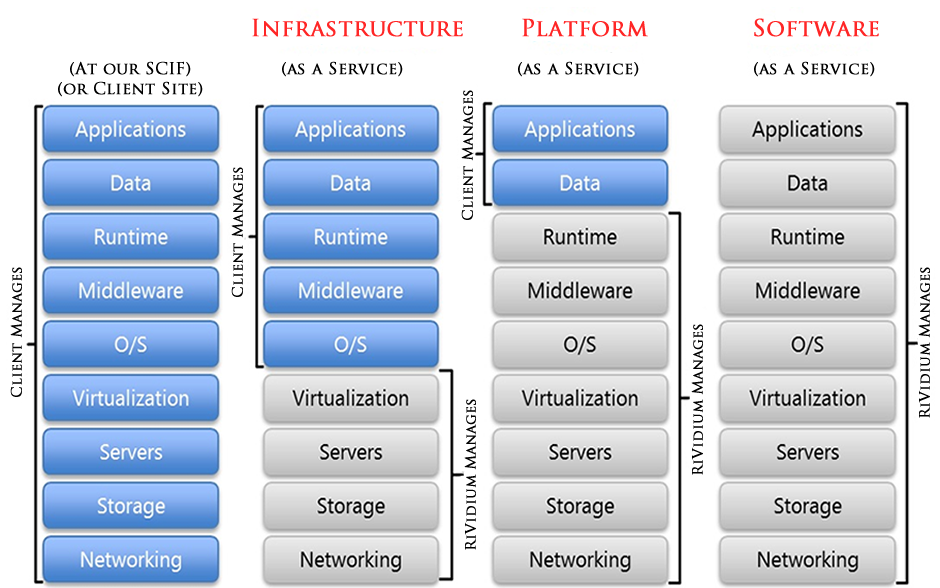
\includegraphics[width=12cm]{./images/cloud-models.png}
	\caption{Modelos de nubes} \label{fig:cloud-models}
\end{figure}

\vspace*{0.2in}
\section{Heroku}\label{cap.3.1}

\vspace*{0.2in}
\section{OpenShift}\label{cap.3.2}
